\section{Personas}
This part will show three different personas.

\subsection{Henrik Jensen}
\begin{figure}[H]
	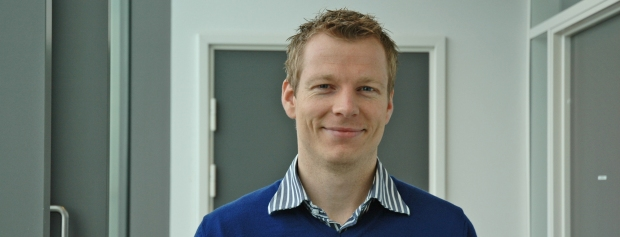
\includegraphics[width=0.30\textwidth]{Grafik/FoodPlanner/PersonaHenrikJensen}
	\label{PersonaHenrikJensen}
\end{figure}
\begin{itemize}
	\item Age: 38
	\item Relational status: Married
	\item Children: 2, age 16 and 14
	\item Occupation: Working as an IT consultant.
	\item Preferences: Wanna spend less time on shopping but still cook delicious dinners.
\end{itemize}
-Henrik drives home after he has finished a meeting with a costumer. The meeting dragged on and Henrik Just want to get home and get a nice dinner.

-His wife is working as a nurse and has a late night shift this evening. It is therefore up to Henrik to cook Dinner for the whole family

-On his way home he stops by the local supermarket and on his way to the entrance he starts to plan what he will prepare for dinner.

-He finds some meat on sale which he decides to buy.

-When he gets home he finds the recipe he wanted and starts to cook.

-It annoys him slightly that he does not plan ahead and very variated. Bu he fells he ha no other choice because of his work schedule and his desire to reduce shopping time.

-After dinner he starts the washing machine and turns on tv to watch football. He is an football enthusiast and played it himself when he was younger. 

\subsection{Peter Nielsen}
\begin{figure}[H]
	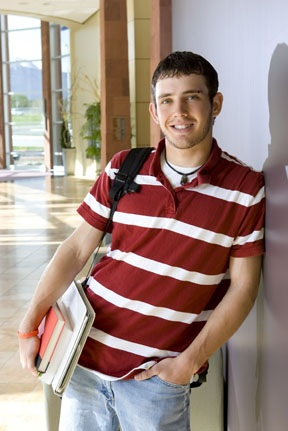
\includegraphics[width=0.15\textwidth]{Grafik/FoodPlanner/PersonaPeterNielsen}
	\label{PersonaHenrikJensen}
\end{figure}
\begin{itemize}
	\item Age: 23
	\item Relational status: Single
	\item Children: None
	\item Occupation: Student
	\item Preferences: Does not spend more time in the kitchen than needed.
\end{itemize}
-Peter has classes till late afternoon, so when he gets of school he rushes home, and does not care about dinner when he leaves school.

-Peter first plans what he is going to have for dinner when he get home. At this point he is usually just plans something that is fast to make.

-When he has to shop he goes for the nearest shop, and just buys what the recipe says, and does not look at what is on sale.

-When he gets home after buying the ingredients, he wait till he is hungry before starting making the food.

-He is slightly annoyed that he does not plan ahead but he blames that he has no things to help him seclude his plans.

-After dinner he starts he goes sit in front of the computer where he starts playing video games with his friends.

\subsection{Anne Madsen}
\begin{figure}[H]
	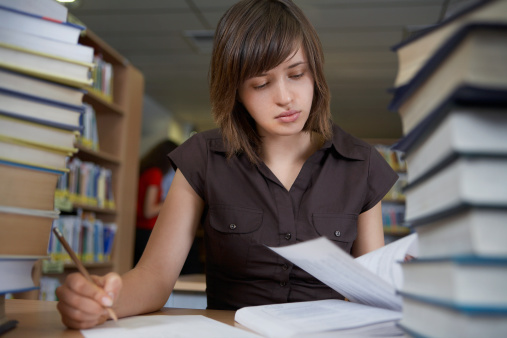
\includegraphics[width=0.25\textwidth]{Grafik/FoodPlanner/PersonaAnneMadsen}
	\label{PersonaHenrikJensen}
\end{figure}
\begin{itemize}
	\item Age: 18
	\item Relational status: Single
	\item Children: None
	\item Occupation: Student
	\item Preferences: Likes to spend time in the kitchen to prepare a good fresh meal with vegetables
\end{itemize}
-Anne has classes till late afternoon, after school Anne has a specific shopping list based on what she has to buy to make food for dinner.

-Anne does not know where to find the cheapest groceries which she finds slightly annoying, so she keeps shopping the same place as she has always done.

-When Anne is done shopping she decides that it is too dangerous to ride her bike with a bag of groceries hanging of her handlebar. So she decides to pull her bike home.

-When Anne finally gets home the trip from school to home has taken so long that it is time to make dinner.

-After dinner she cleans the plates, and gets ready to prepare her homework for the next day. 
